% ===== Section 3: "Empty vessels make the most noise" (~15 min) =====
\topicopener{loudspeaker}{Վստահություն}{Դատարկ տակառն է շատ ձայն հանում}{Ինչու են խելացի մարդիկ հաճախ պարտվում վեճերում}{angry}

% An argument you cannot win: "It's twenty fifteen? Duh!"
\begin{frame}{Վեճ, որ հնարավոր չէ հաղթել}
  \begin{columns}[c]
    \begin{column}{0.46\textwidth}
      Ամենանյարդայնացնող բաներից մեկը՝ վիճել մեկի հետ, ով համոզված է, որ ճիշտ է, թեև փաստերով ու տրամաբանությամբ կարող ես ապացուցել հակառակը։\par\medskip
      Բըրնեթը մի անգամ ականատես է եղել այսպիսի վեճի.
    \end{column}
    \begin{column}{0.5\textwidth}
      \begin{tikzpicture}
        \node[chatmsg=4.6cm, fill=peach!45!cardwhite, anchor=west, visible on=<2->] (a) at (0,0) {Հիմա 20-րդ դարն է, ոչ թե 21-րդը։};
        \node[chatmsg=4.6cm, fill=mint!40!cardwhite, anchor=east, visible on=<3->] (b) at (6,-1.15) {21-րդն է...};
        \node[chatmsg=4.6cm, fill=peach!45!cardwhite, anchor=west, visible on=<4->] (c) at (0,-2.3) {It's \textbf{twenty} fifteen, չէ՞։ \textbf{Դե՜}};
        \node[anchor=north, visible on=<5->] at (4.6,-2.7) {\showon{5-}{\mascot[1.6cm]{angry}}};
      \end{tikzpicture}
    \end{column}
  \end{columns}
  \vspace{2mm}
  \onslide<5->{\centering\small Ամբողջ փաստարկն այդ էր (անգլերենում 2015-ը «twenty fifteen» է)։\par}
\end{frame}

% Impostor syndrome + poll
\begin{frame}{Խաբեբայի համախտանիշ (impostor syndrome)}
  \begin{columns}[T]
    \begin{column}{0.54\textwidth}
      \begin{itemize}
        \item Հաջողակ մարդիկ համառորեն \textbf{թերագնահատում} են իրենց ունակությունները՝ չնայած ապացույցներին
        \item<2-> Հաճախ է «տղամարդկային» ոլորտներում հաջողած կանանց մոտ. կարծրատիպեր, նախապաշարմունքներ
        \item<3-> Բայց ոչ միայն նրանց մոտ, ու հիմնականում հենց \textbf{խելացիների} մոտ
      \end{itemize}
    \end{column}
    \begin{column}{0.42\textwidth}
      \onslide<4->{%
      \begin{poll}
        Բարձրացրու ձեռքդ, եթե մտածել ես. «Ինձ պատահմամբ են ընդունել, շուտով բոլորը կհասկանան»։
      \end{poll}}
      \onslide<5->{%
      \begin{card}[colback=mint!35!cardwhite]
        Եթե այո, լավ ընկերակցության մեջ ես։ Հաջորդ սլայդում՝ ում։
      \end{card}}
    \end{column}
  \end{columns}
\end{frame}

% Guess who said it: Einstein
\begin{frame}{Գուշակիր՝ ով է ասել}
  \begin{columns}[c]
    \begin{column}{0.6\textwidth}
      \begin{bookquote}
        Իմ կյանքի գործի չափազանցված գնահատականն ինձ շատ անհարմար է զգացնում։ Ստիպված եմ ինձ \textbf{ակամա խաբեբա} համարել։
      \end{bookquote}
      \vspace{1mm}
      \begin{chatbox}
        \textbf{Ա}՝ Նյուտոն, \textbf{Բ}՝ Մարի Կյուրի, \textbf{Գ}՝ Այնշտայն, \textbf{Դ}՝ Հոքինգ
      \end{chatbox}
    \end{column}
    \begin{column}{0.34\textwidth}
      \centering
      \onslide<2->{%
      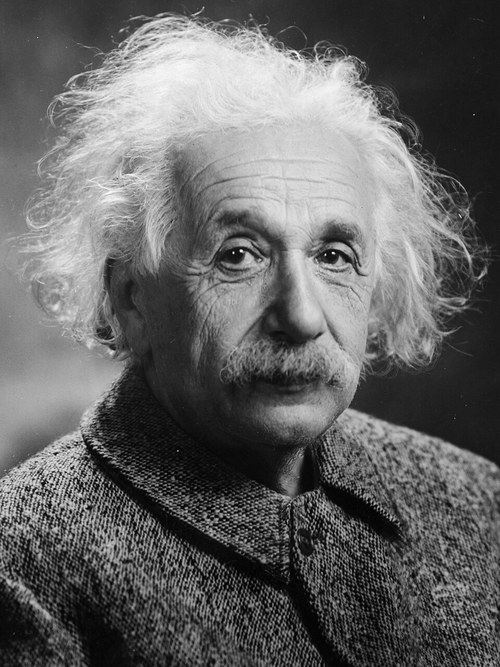
\includegraphics[height=3.6cm]{einstein.jpg}\par\smallskip
      {\small \textbf{Ալբերտ Այնշտայն}, մահից քիչ առաջ։\par Ամենևին էլ «թույլ աշակերտ» չէր։\par}}
    \end{column}
  \end{columns}
\end{frame}

% Confident witnesses win
\begin{frame}{Վստահ ձայնն ավելի համոզիչ է}
  \begin{columns}[c]
    \begin{column}{0.5\textwidth}
      \begin{itemize}
        \item Տեղեկության ու աջակցության համար ապավինում ենք ուրիշներին (մանրամասն՝ գլուխ 7-ում)
        \item<2-> Որքան \textbf{վստահ} է խոսողը, այնքան ավելի են նրան հավատում
        \item<3-> 1990-ականներ, Փենրոդ և Քաթլեր. երդվյալ ատենակալներն ավելի շատ էին հավատում վստահ վկաներին, քան նյարդայիններին
        \item<4-> Ասելու \textbf{ձևն} ավելի կարևոր էր, քան \textbf{բովանդակությունը}
      \end{itemize}
    \end{column}
    \begin{column}{0.46\textwidth}
      \centering
      \begin{tikzpicture}
        \node at (0,0) {\bigemoji[1.2cm]{judge}};
        \node[wbubble=3.8cm, font=\handfont\normalsize, visible on=<3->, fill=mint!35!cardwhite] at (0,1.6) {Հաստա՛տ նա էր։ Հարյուր տոկոսով։};
        \node[wbubble=3.8cm, font=\handfont\normalsize, visible on=<3->, fill=peach!40!cardwhite] at (0,-1.6) {Կարծեմ... գուցե նա էր... չեմ հիշում...};
        \node[font=\Large, visible on=<4->] at (2.5,1.6) {\showon{4-}{\emoji{check}}};
        \node[font=\Large, visible on=<4->] at (2.5,-1.6) {\showon{4-}{\emoji{cross}}};
      \end{tikzpicture}
    \end{column}
  \end{columns}
\end{frame}

% Politics and public debate
\begin{frame}{Քաղաքականությունն ու հանրային վեճերը}
  \begin{columns}[c]
    \begin{column}{0.56\textwidth}
      \begin{itemize}
        \item Պատվաստումների ու կլիմայի մասին վեճերում հաճախ իշխում են \textbf{չտեղեկացվածների} կրքոտ ելույթները, ոչ թե մասնագետների հանգիստ բացատրությունները
        \item<2-> Քաղաքական գործիչներին սովորեցնում են վստահ խոսել ցանկացած թեմայով՝ առանց արժեքավոր բան ասելու
        \item<3-> Որքան խելացի է մարդը, այնքան հաճախ է \textbf{կասկածում}, իսկ կասկածողին քիչ են վստահում
      \end{itemize}
    \end{column}
    \begin{column}{0.38\textwidth}
      \centering
      \onslide<2->{%
      \begin{card}[colback=lavender!35!cardwhite]
        {\blackfont\large «They misunderestimated me»}\par\smallskip
        {\small Ջորջ Բուշ. «misunderstood» ու «underestimated» մեկ բառի մեջ}
      \end{card}}
      \onslide<3->{%
      \begin{bookquote}
        Ահա՛ ձեզ ժողովրդավարություն։
      \end{bookquote}}
    \end{column}
  \end{columns}
\end{frame}

% The chapter title: "Oh, think you're clever, do you?"
\begin{frame}{«Կարծում ես՝ խելացի՞ ես»}
  \begin{columns}[T]
    \begin{column}{0.47\textwidth}
      \begin{tikzpicture}
        \node[chatmsg=4.4cm, fill=cardwhite, anchor=west] (a) at (0,0) {Ինչո՞վ ես զբաղվում։};
        \node[chatmsg=4.4cm, fill=mint!40!cardwhite, anchor=east] (b) at (5.9,-1.0) {Նեյրոգիտնական եմ։};
        \node[chatmsg=4.4cm, fill=peach!45!cardwhite, anchor=west, visible on=<2->] (c) at (0,-2.0) {Հա՛... \textbf{Կարծում ես՝ խելացի՞ ես}};
      \end{tikzpicture}
    \end{column}
    \begin{column}{0.47\textwidth}
      \onslide<3->{%
      \begin{tikzpicture}
        \node[chatmsg=4.4cm, fill=cardwhite, anchor=west] (a) at (0,0) {Ինչո՞վ ես զբաղվում։};
        \node[chatmsg=4.4cm, fill=mint!40!cardwhite, anchor=east] (b) at (5.9,-1.0) {Օլիմպիական վազորդ եմ։};
        \node[chatmsg=4.4cm, fill=peach!45!cardwhite, anchor=west] (c) at (0,-2.0) {Հա՛... Կարծում ես՝ արա՞գ ես};
        \draw[pinkdark, line width=2pt] (c.south west) -- (c.north east);
      \end{tikzpicture}}
    \end{column}
  \end{columns}
  \vspace{4mm}
  \onslide<4->{%
  \begin{bookquote}
    Ուստի հիմա ասում եմ. «Նեյրոգիտնական եմ, բայց դա այնքան տպավորիչ չէ, որքան հնչում է»։
  \end{bookquote}}
\end{frame}

% Why we are suspicious of clever people
\begin{frame}{Ինչու ենք կասկածանքով նայում խելացիներին}
  \begin{columns}[T]
    \begin{column}{0.47\textwidth}
      \begin{card}[colback=mint!35!cardwhite]
        \centering\bigemoji[1cm]{weightlifter}\par\smallskip
        \raggedright{\blackfont Ուժեղ մարդը հասկանալի է}\par\smallskip
        Շատ է մարզվում։ Ով էլ նույնն անի, նրա պես կդառնա։ Կշռաքարը բազուկ է տալիս, պարզ է։
      \end{card}
    \end{column}
    \begin{column}{0.47\textwidth}
      \onslide<2->{%
      \begin{card}[colback=brainpink!25!cardwhite]
        \centering\bigemoji[1cm]{nerd}\par\smallskip
        \raggedright{\blackfont Քեզնից խելացին անհայտ է}\par\smallskip
        Չես կարող կանխատեսել նրա քայլերը։ Իսկ սովորելու ու խելքի կապը շատ ավելի մշուշոտ է։
      \end{card}}
    \end{column}
  \end{columns}
  \vspace{2mm}
  \onslide<3->{%
  \begin{card}[colback=butter!45!cream]
    Ուղեղը չի կարող որոշել՝ վտանգավո՞ր է, թե՞ ոչ, ու միանում է հին բնազդը. \textbf{«ավելի լավ է ապահով, քան ափսոս»}։ Արդյունքը՝ կասկած ու թշնամանք։
  \end{card}}
\end{frame}

% The lemon-juice bank robber
\begin{frame}{Լիմոնի հյութով կողոպուտը}
  \begin{columns}[c]
    \begin{column}{0.56\textwidth}
      \begin{enumerate}
        \item<1-> Մի մարդ կողոպտում է բանկեր՝ դեմքին \textbf{լիմոնի հյութ} քսած
        \item<2-> Նրա տրամաբանությունը. լիմոնի հյութով «անտեսանելի թանաք» են սարքում, ուրեմն տեսախցիկն էլ դեմքը չի տեսնի
        \item<3-> Տեսախցիկը, իհարկե, տեսավ \emoji{camera}
        \item<4-> Այս պատմությունը ոգեշնչեց Քորնելի համալսարանի երկու հոգեբանի
      \end{enumerate}
    \end{column}
    \begin{column}{0.38\textwidth}
      \centering
      \bigemoji[1.5cm]{lemon}\ \raisebox{0.5cm}{\Large$\rightarrow$}\ \bigemoji[1.5cm]{ghost}\ \raisebox{0.5cm}{\Large ?}\par\medskip
      \onslide<3->{%
      \begin{bookquote}
        Մի պահ թողեք, որ սա «նստի»։
      \end{bookquote}}
    \end{column}
  \end{columns}
  \source{Pant, 2014 (գրքի ծանոթագրությունից)}
\end{frame}

% Meme: Change My Mind, the lemon-juice logic
\begin{frame}{Անտեսանելիության գաղտնիքը}
  \centering
  \begin{meme}[8.2cm]{change_my_mind.jpg}
    \memecap[text width=3.5cm, font=\blackfont\footnotesize]{0.655}{0.31}{Լիմոնի հյութը ինձ անտեսանելի է դարձնում տեսախցիկների համար}
    \memecap[minimum width=3.6cm, font=\blackfont\footnotesize]{0.655}{0.09}{ՓՈԽԻՐ ԿԱՐԾԻՔՍ}
  \end{meme}
\end{frame}

% The Dunning-Kruger effect
\begin{frame}{Դանինգ-Կրյուգերի էֆեկտը}
  \begin{columns}[c]
    \begin{column}{0.42\textwidth}
      Դեյվիդ Դանինգն ու Ջասթին Կրյուգերը մասնակիցներին թեստեր տվեցին ու խնդրեցին գնահատել, թե \textbf{որքան լավ} են գրել։\par\medskip
      \onslide<2->{\textbf{Ամենաթույլերը} կարծում էին, որ միջինից լավ են գրել։\par\smallskip}
      \onslide<3->{\textbf{Ամենաուժեղները} իրենց մի փոքր թերագնահատում էին։\par}
    \end{column}
    \begin{column}{0.54\textwidth}
      \centering
      \onslide<2->{% Kruger & Dunning (1999), Study 2 (logical reasoning), percentile of test score:
% bottom quartile actual 12th, estimated 62nd; top quartile actual 86th, estimated 68th.
\begin{tikzpicture}
  \begin{axis}[
      width=7.6cm, height=5.0cm,
      ybar, bar width=0.85cm,
      ymin=0, ymax=100,
      symbolic x coords={bottom, top},
      xtick={bottom, top},
      xticklabels={{Ամենաթույլ\\ քառորդը}, {Ամենաուժեղ\\ քառորդը}},
      xticklabel style={align=center, font=\small, text=plum},
      ytick={0,50,100}, yticklabel={\pgfmathprintnumber{\tick}},
      tick label style={font=\small, text=plum}, axis line style={plum},
      axis x line*=bottom, axis y line*=left, ymajorgrids, grid style={plum!10},
      ylabel={պերցենտիլ}, ylabel style={font=\small, text=plum},
      nodes near coords, nodes near coords style={font=\blackfont\small, text=plum},
      enlarge x limits=0.45,
      legend style={draw=none, fill=none, font=\small, text=plum, at={(0.5,1.02)}, anchor=south, legend columns=2,
        /tikz/every even column/.append style={column sep=4mm}},
      legend image code/.code={\fill[#1] (0cm,-0.1cm) rectangle (0.3cm,0.15cm);},
    ]
    \addplot[fill=amBlue, draw=none] coordinates {(bottom,12) (top,86)};
    \addplot[fill=amOrange, draw=none] coordinates {(bottom,62) (top,68)};
    \legend{իրականում, իրենց կարծիքով}
  \end{axis}
\end{tikzpicture}
\par}
      {\scriptsize\color{plum!70!cream} տրամաբանության թեստ. 100-ը՝ ամենալավ արդյունքը\par}
    \end{column}
  \end{columns}
  \source{Kruger \& Dunning, J. Pers. Soc. Psychol., 1999, հետազոտություն 2}
\end{frame}

% Why: the two sides
\begin{frame}{Ինչու՞ է այդպես}
  \begin{columns}[T]
    \begin{column}{0.47\textwidth}
      \begin{card}[colback=peach!40!cardwhite]
        {\blackfont Քիչ գիտեցողները}\par\smallskip
        \begin{itemize}\small
          \item Սեփական սխալը տեսնելու համար պետք է \textbf{հենց այն հմտությունը}, որը պակասում է
          \item Ուղեղը կարծում է՝ բոլորը մեզ նման են. ինչպես գունակույրին խնդրել նկարագրել կարմիր-կանաչ նախշը
        \end{itemize}
      \end{card}
    \end{column}
    \begin{column}{0.47\textwidth}
      \onslide<2->{%
      \begin{card}[colback=lavender!40!cardwhite]
        {\blackfont Շատ գիտեցողները}\par\smallskip
        \begin{itemize}\small
          \item Կարծում են՝ իրենց համար հեշտը բոլորի համար է հեշտ
          \item Գիտեն, թե \textbf{որքան բան չգիտեն}
          \item Շրջապատված են խելացիներով, որոնք կնկատեն ամեն սխալ
        \end{itemize}
      \end{card}}
    \end{column}
  \end{columns}
  \vspace{2mm}
  \onslide<3->{\centering\small Զգուշությունը գիտության մեջ առավելություն է, իսկ վեճում՝ \textbf{թուլություն}։\par}
\end{frame}

% Science update: statistical critiques of Dunning-Kruger
\begin{frame}{Դանինգ-Կրյուգեր. ինչ գիտենք այսօր}
  \begin{columns}[c]
    \begin{column}{0.64\textwidth}
      \begin{scienceupdate}
        \begin{itemize}\setlength{\itemsep}{0.6mm}
          \item Էֆեկտը կոնկրետ \textbf{հմտության} մասին է (տրամաբանություն, քերականություն, հումոր), ոչ թե «ցածր IQ»-ի
          \item Նույն պատկերի մի մասը ստացվում է \textbf{նույնիսկ պատահական թվերից}. բոլորն իրենց մի փոքր միջինից լավ են համարում, իսկ ծայրերը «ձգվում» են դեպի միջինը (regression to the mean)
          \item Թույլերի գերագնահատումն իրական է, իսկ դրա պատճառը դեռ վիճելի է
        \end{itemize}
      \end{scienceupdate}
    \end{column}
    \begin{column}{0.3\textwidth}
      \centering
      \mascot[2.0cm]{thinking}\par\smallskip
      {\small Համացանցի «Հիմարության գագաթ» գրաֆիկը Դանինգի ու Կրյուգերի հոդվածում \textbf{չկա}։\par}
    \end{column}
  \end{columns}
  \source{Nuhfer et al., Numeracy, 2016; Gignac \& Zajenkowski, Intelligence, 2020}
\end{frame}

% Not everyone; culture
\begin{frame}{Ոչ բոլորն են այդպես}
  \begin{columns}[c]
    \begin{column}{0.56\textwidth}
      \begin{itemize}
        \item Ոչ ամեն խելացի է կասկածներով լի, ու ոչ ամեն քիչ գիտեցող է ինքնագոհ
        \item<2-> Կան ինտելեկտուալներ, որ այնքան են սիրում իրենց ձայնը, որ հազարներ են գանձում այն լսելու համար
        \item<3-> Կան քիչ գիտեցողներ, որ համեստորեն ընդունում են դա
      \end{itemize}
    \end{column}
    \begin{column}{0.4\textwidth}
      \onslide<4->{%
      \begin{card}[colback=mint!35!cardwhite]
        \emoji[1.3em]{earth}\ {\blackfont Մշակույթն էլ է կարևոր}\par\smallskip
        Հետազոտությունները հիմնականում արևմտյան են։ Արևելյան Ասիայի որոշ մշակույթներում չիմացածը համարում են \textbf{զարգանալու հնարավորություն}, ու պատկերն այլ է։
      \end{card}}
    \end{column}
  \end{columns}
  \source{DeAngelis, APA Monitor, 2003}
\end{frame}

% The brain behind self-appraisal
\begin{frame}{«Լա՞վ եմ անում». ուղեղի պատասխանը}
  \begin{columns}[c]
    \begin{column}{0.54\textwidth}
      \begin{itemize}
        \item 2009. Հովարդ Ռոզենի խումբը ուսումնասիրեց նեյրոդեգեներատիվ հիվանդությամբ \textbf{մոտ 40 պացիենտի}
        \item<2-> Ինքնագնահատման ճշգրտությունը կապված էր նախաճակատային կեղևի \textbf{աջ ներքին-ստորին} հատվածի (right ventromedial PFC) ծավալի հետ
        \item<3-> 40 մարդը քիչ է բոլորի մասին եզրակացնելու համար
      \end{itemize}
    \end{column}
    \begin{column}{0.42\textwidth}
      \centering
      \begin{tikzpicture}[scale=0.68]
        \brainbg
        \brainlines
        \filldraw[fill=amRed!50!cream, draw=pinkdark, line width=0.8pt, dashed, visible on=<2->] (0.85,1.35) ellipse (0.55 and 0.32);
        \node[font=\scriptsize, text=plum, align=center, anchor=north, visible on=<2->] (v) at (0.2,0.55) {ներքին-ստորին\\ հատված};
      \end{tikzpicture}\par
      \onslide<4->{%
      \begin{card}[colback=butter!45!cream]
        \textbf{Մետաճանաչողություն} (metacognition)՝ մտածել սեփական մտածողության մասին։
      \end{card}}
    \end{column}
  \end{columns}
  \source{Rosen et al., NeuroImage, 2010}
\end{frame}

% When self-appraisal breaks; confident clowns
\begin{frame}{Վստահ ծաղրածուներ ու անվստահ ինտելեկտուալներ}
  \begin{columns}[T]
    \begin{column}{0.52\textwidth}
      \begin{itemize}
        \item Ինքնագնահատման խանգարումը դեմենցիայի նշան է, հատկապես \textbf{ճակատաքունքային դեմենցիայի} (frontotemporal dementia), որը վնասում է հիմնականում ճակատային բիլթը
        \item<2-> Ոմանք կարծում են՝ դրանով է բացատրվում պացիենտների ագրեսիան. չեն կարողանում անել ու չեն հասկանում՝ ինչու
      \end{itemize}
    \end{column}
    \begin{column}{0.42\textwidth}
      \onslide<3->{Առողջ ուղեղն էլ միայն \textbf{հնարավորություն} է տալիս գնահատել ինքդ քեզ, ոչ թե երաշխիք, որ գնահատականը ճիշտ կլինի։\par\medskip}
      \onslide<4->{%
      \begin{bookquote}
        Արդյունքում՝ վստահ ծաղրածուներ ու անվստահ ինտելեկտուալներ։ Ու մենք լսում ենք վստահներին։
      \end{bookquote}}
    \end{column}
  \end{columns}
\end{frame}
